%%%%%%%%%%%%%%%%%%%%%%%%%%%%%%%%%%%%%%%%%%%%%
%% Introdução ao protocolo TLS
%% Copyright 2006 Eliézio Batista de Oliveira
%%%%%%%%%%%%%%%%%%%%%%%%%%%%%%%%%%%%%%%%%%%%%

\chapter{Introdução ao protocolo TLS}

É apresentada a seguir uma descrição básica do protocolo TLS. Uma descrição
completa do protocolo pode ser encontrada na especificação
oficial~\cite{rfc_tls} ou mais detalhadamente no livro \emph{``SSL and
TLS: Designing and Building Secure Systems''}~\cite{Rescorla}.

\section{O criptossistema TLS}
\label{sec:OCriptossistemaTLS}

O TLS é um criptossistema híbrido onde todos os parâmetros dos algoritmos 
simétricos são dinâmicos e derivados de um parâmetro-mestre chamado \emph{master-key},
por sua vez definido através de um \acs{PKA} para o estabelecimento de chave.

No TLS os algoritmos criptográficos não podem ser combinados livremente mas
são pré-arranjados em forma de \emph{ciphersuites}.
Um \emph{ciphersuite} é basicamente uma quádrupla $<Au,Kx,Enc,Mac>$ que denota
respectivamente os algoritmos de autenticação, de estabelecimento de chave, 
de cifragem e a função de \emph{Hashing} usado no cômputo do \acs{HMAC}.

\section{Conexão e Sessão TLS}
\label{sec:ConexãoESessãoTLS}

Uma conexão TLS é um canal transiente estabelecido entre duas aplicações tendo por base 
um protocolo de transporte confiável, tipicamente o \acs{TCP}. Uma conexão tem
fundamentalmente duas fases distintas: \emph{handshake} e transferência de dados
das aplicações (\emph{bulk data transfer}).

O \emph{handshake} TLS possui três propósitos:
\begin{enumerate}
	\item Negociar o \emph{ciphersuite} e os parâmetros da sessão TLS (definida abaixo);
	\item Derivar todos os demais parâmetros criptográficos usados pelos algoritmos 
	simétricos;
	\item Autenticar as partes envolvidas (opcional).
\end{enumerate}

Uma sessão TLS é caracterizada pelos seguintes atributos:

\begin{center}
\begin{tabular}{@{}rp{10cm}@{}} \toprule
	\tm{Version} 		& Versão do protocolo TLS ou SSL. \\
	\addlinespace
	\tm{Session ID} 	& Identificador da sessão, definido pelo servidor. \\
	\addlinespace
	\tm{master-key}		& Chave mestre definida através de um \acs{PKA} para
	o estabelecimento de chave. \\
	\addlinespace
	$<Enc,Mac>$			& Algoritmos de cifragem e MAC, subconjunto do \emph{ciphersuite}. \\
	\addlinespace
	\tm{Compression Method} & Algoritmo de compressão. \\ \bottomrule
\end{tabular}
\end{center}

Uma vez constituída, uma sessão pode ser restaurada nas conexões subseqüentes, economizando
assim o alto custo computacional exigido para seu estabelecimento.

\section{Arquitetura do protocolo TLS}
\label{sec:ArquiteturaDoProtocoloTLS}

O TLS é implementado de modo a atuar entre a camada de aplicação e a de
transporte, como ilustra a Figura~\vref{fig:tls_stack} adaptada
de~\cite{Thomas}.

\begin{figure}[htbp]
    \centering
        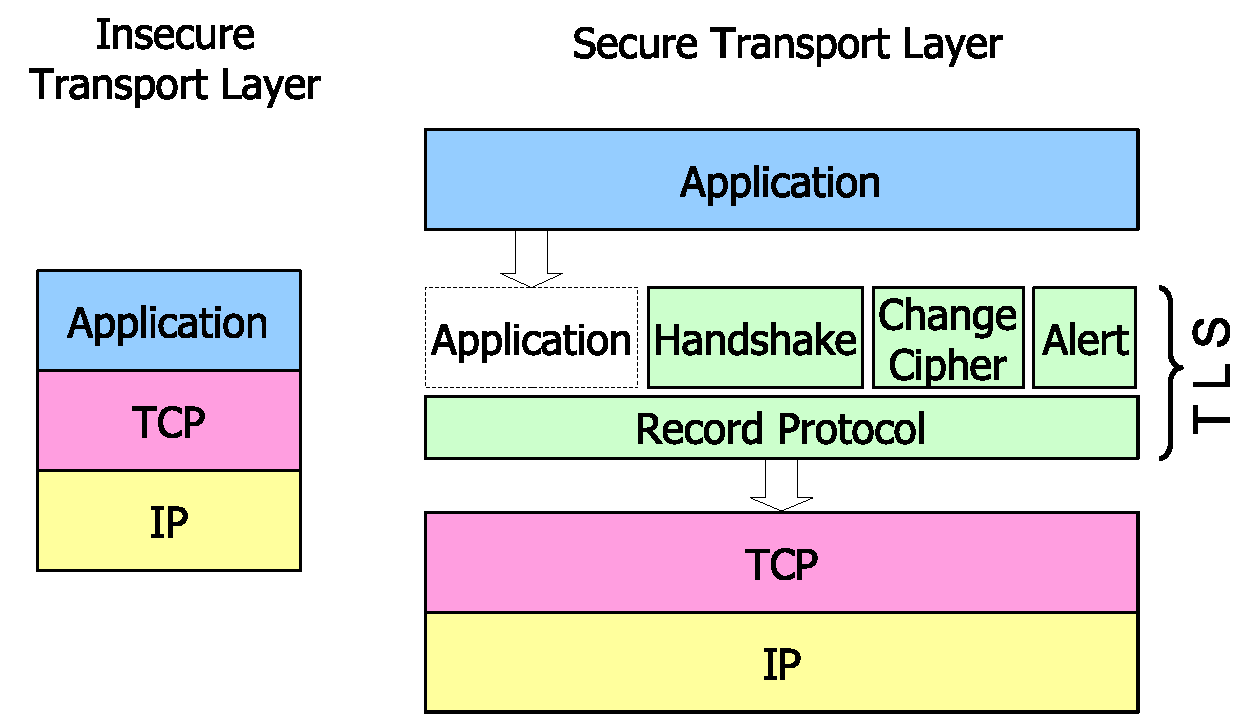
\includegraphics[scale=0.5]{fig/tls_stack}
    \caption{TLS na arquitetura em camadas de protocolos}
    \label{fig:tls_stack}
\end{figure}

O TLS pode ser decomposto em quatro sub-protocolos dispostos em duas camadas,
sendo um inferior, chamado de \emph{Record Protocol} e três superiores a saber:
\emph{Handshake}, \emph{Alert} e \emph{Change Cipher Spec} (CCS).

Do ponto de vista funcional, o CCS, composto de uma única mensagem homônima, é
parte integrante do \emph{handshake} e assim será abordado neste texto. A sua
discriminação como um protocolo em separado serve apenas ao único propósito de
garantir que a sua mensagem não compartilhe o mesmo registro com as demais
mensagens do \emph{handshake}.

\subsection{\emph{TLS Record Protocol}}

Um registro TLS encapsula uma ou mais mensagens recebidas de um dos
quatro protocolos superiores, e processadas conforme os mesmos parâmetros 
criptográficos correntes na conexão TLS. 

Conforme exposto na Figura~\vref{fig:tls_rec_protocol},
toda mensagem oriunda das camadas superiores é primeiramente
fragmentada em blocos de até $2^{14}$ bytes (16 kB), sendo eventualmente
comprimida em seguida\footnote{A RFC~2246 não especifica nenhum
algoritmo de compressão.}.

\begin{figure}[htbp]
    \centering
        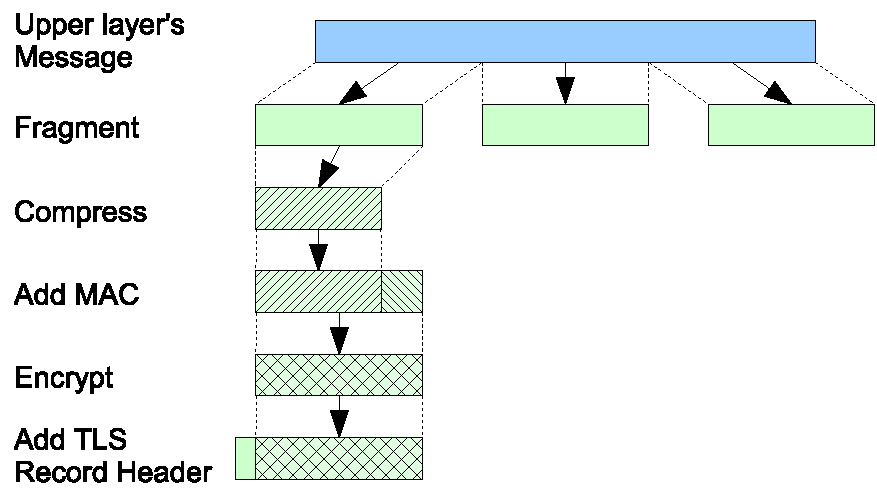
\includegraphics[scale=0.7]{fig/tls_rec_protocol}
    \caption{\emph{TLS Record Protocol}}
    \label{fig:tls_rec_protocol}
\end{figure}

O próximo estágio no processamento da mensagem é o cálculo e o acréscimo do seu
\acs{MAC}, provendo assim a verificabilidade da integridade da mensagem e da
autenticidade da sua origem.

Se o cifrador corrente for do tipo \emph{block cipher}, acrescenta-se tantos
bytes extras quanto forem necessários até que a soma do fragmento comprimido mais
o MAC seja um múltiplo inteiro do tamanho do bloco do cifrador.

Finalmente ocorre a cifragem de toda a mensagem concatenada ao seu \acs{MAC}
usando um cifrador simétrico, sendo em seguida prefixada por um \emph{header}
de cinco bytes ilustrado na Figura~\vref{fig:tls_rec_header} e descrito na Tabela~\vref{tab:TLSRecordHeader}.

\begin{figure}[htbp]
	\centering
		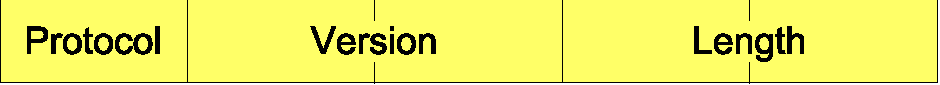
\includegraphics[scale=0.4]{fig/tls_rec_header}
	\caption{\emph{TLS Record Header}}
	\label{fig:tls_rec_header}
\end{figure}

\begin{table}[htbp]
	\centering
		\begin{tabular}{@{}lcp{10cm}@{}} \toprule
		\tm{Campo} & \tm{Tamanho} & \tm{Descrição} \\ \midrule
		\emph{Protocol} & 1 & Indica o protocolo superior das mensagens encapsuladas
						 segundo a seguinte codificação:
						\begin{center}
						\begin{tabular}{@{}cl@{}}
						 \tm{Tipo} & \tm{Protocolo} \\ \midrule
							20 & \tlsHsCcs \\
							21 & \emph{Alert} \\
							22 & \emph{Handshake} \\
							23 & \emph{Application Data} \\
						\end{tabular}
						\end{center} \\
		\emph{Version} & 2 & Versão do protocolo. A versão 1.0 do TLS é codificada 
							 como \verb|03 01| (em hexadecimal). \\
		\addlinespace
		\emph{Length}  & 2 & Tamanho total do conteúdo do registro, não podendo exceder a $2^{14} + 2048$. \\ \bottomrule
		\end{tabular}
	\caption{\emph{TLS Record Header}}
	\label{tab:TLSRecordHeader}
\end{table}

O \emph{ciphersuite} ativo no início de uma conexão é o $<NULL,NULL,NULL,NULL>$.

\subsection{\emph{Alert Protocol}}

A única mensagem que compõe esse protocolo pode ser enviada assincronamente por 
qualquer uma das partes para notificar erros para o outro par.

\subsection{\emph{Handshake Protocol}}

O \emph{handshake}, por ser o estágio certamente mais complexo, será analisado
mais detalhadamente a seguir através da análise de três casos típicos.

Para evitar aspectos do protocolo TLS desnecessários tendo em vista o escopo 
deste projeto, o \acs{RSA} será o PKA para o estabelecimento de chave empregado
em todos os \emph{handshakes} que se seguem.

\subsubsection{\emph{Handshake} com autenticação do servidor}

A autenticação do servidor é realizada em praticamente todas as negociações
TLS. A Tabela~\vref{tab:hs_server_auth} sumariza cada uma das mensagens
exibidas na Figura~\ref{fig:hs_server_auth}.


\begin{figure}[htp]
    \centering
        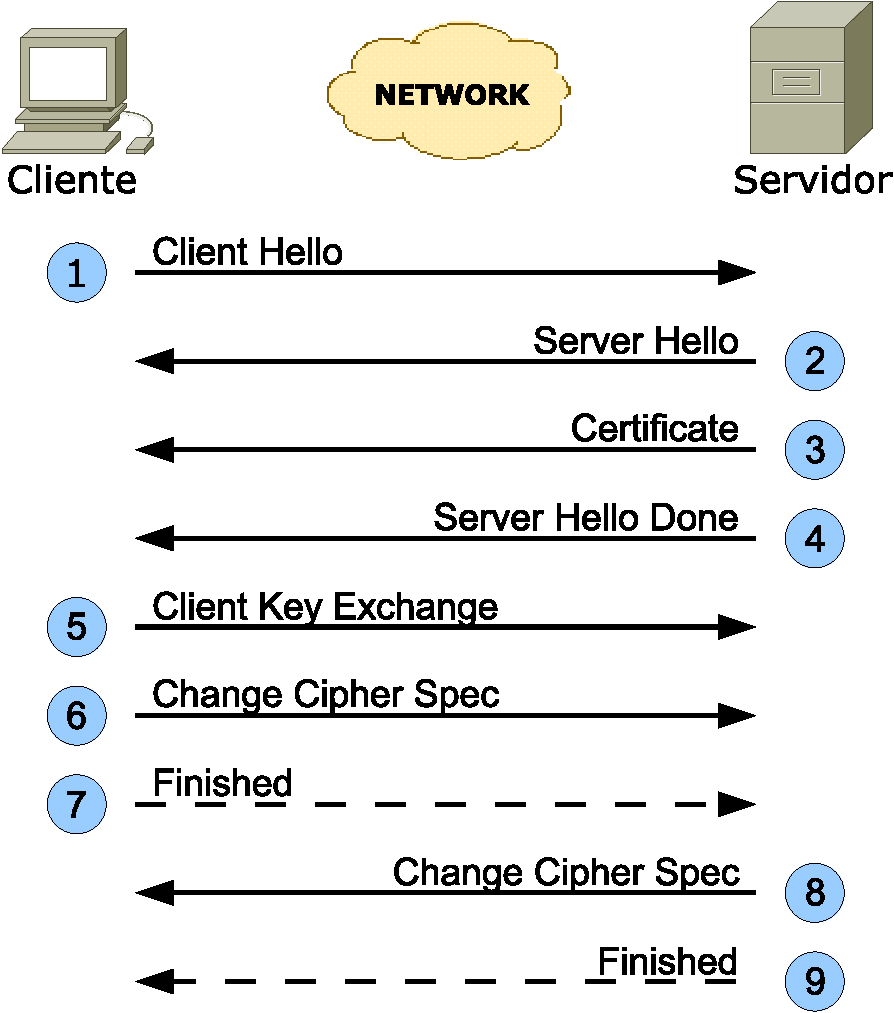
\includegraphics[scale=0.5]{fig/hs_server_auth}
    \caption{\emph{Handshake} completo com autenticação do servidor}
    \label{fig:hs_server_auth}
\end{figure}

\begin{table}[htp]
    \begin{center}
    \caption{\emph{Handshake} completo com autenticação do servidor}
    \label{tab:hs_server_auth}
    \begin{tabular}{@{}lp{15cm}@{}} \toprule
        \tm{\#} & \tm{Descrição} \\ \midrule
1 &
O cliente envia a mensagem \tlsHsCh propondo os seguintes parâmetros
para a conexão:
\begin{itemize}
\item \emph{Version} -- Versão máxima do protocolo suportada (3.1 para o caso do
TLS 1.0);
\item \emph{Nonce} -- Um número (pseudo-) aleatório de 32 bytes recém gerado
para esta conexão;
\item \emph{Session ID} -- Identificador de uma sessão previamente estabelecida,
caso o cliente deseje restaurá-la;
\item \emph{Cipher Suites} -- Lista dos parâmetros criptográficos suportados pelo
cliente;
\item \emph{Compression Methods} -- Lista dos métodos de compressão suportados.
\end{itemize} \\

2 &
Servidor responde com \tlsHsSh selecionando os parâmetros dentre
aqueles propostos pelo cliente e incluindo o seu próprio \emph{Nonce}. \\
\addlinespace
3 &
Servidor envia seu certificado e todos os intermediários que porventura
existam. \\
\addlinespace
4 &
O servidor conclui esse primeiro estágio de negociação com a mensagem
\tlsHsShd. \\
\addlinespace
5 &
O cliente gera uma chave de sessão aleatória e a envia cifrada com a chave
pública do servidor na mensagem \tlsHsCke. \\
\addlinespace
6 &
Através da mensagem \tlsHsCcs o cliente efetiva os parâmetros
criptográficos já acordados. Todas as mensagens subseqüentes passam a ser
cifradas conforme esses novos parâmetros. \\
\addlinespace
7 &
Um \emph{hash} de todas as mensagens enviadas e recebidas é enviado para o
servidor para evitar que negociação não sofra nenhuma interferência
indevida. \\
\addlinespace
8 &
O servidor também efetiva os parâmetros recém-negociados. \\
\addlinespace
9 &
O servidor envia o \emph{hash} calculado sobre as mensagens enviadas e recebidas
para reforçar a integridade da negociação. \\ \bottomrule
    \end{tabular}
    \end{center}
\end{table}

\subsubsection{\emph{Handshake} com autenticação mútua}

\begin{figure}[htp]
    \centering
        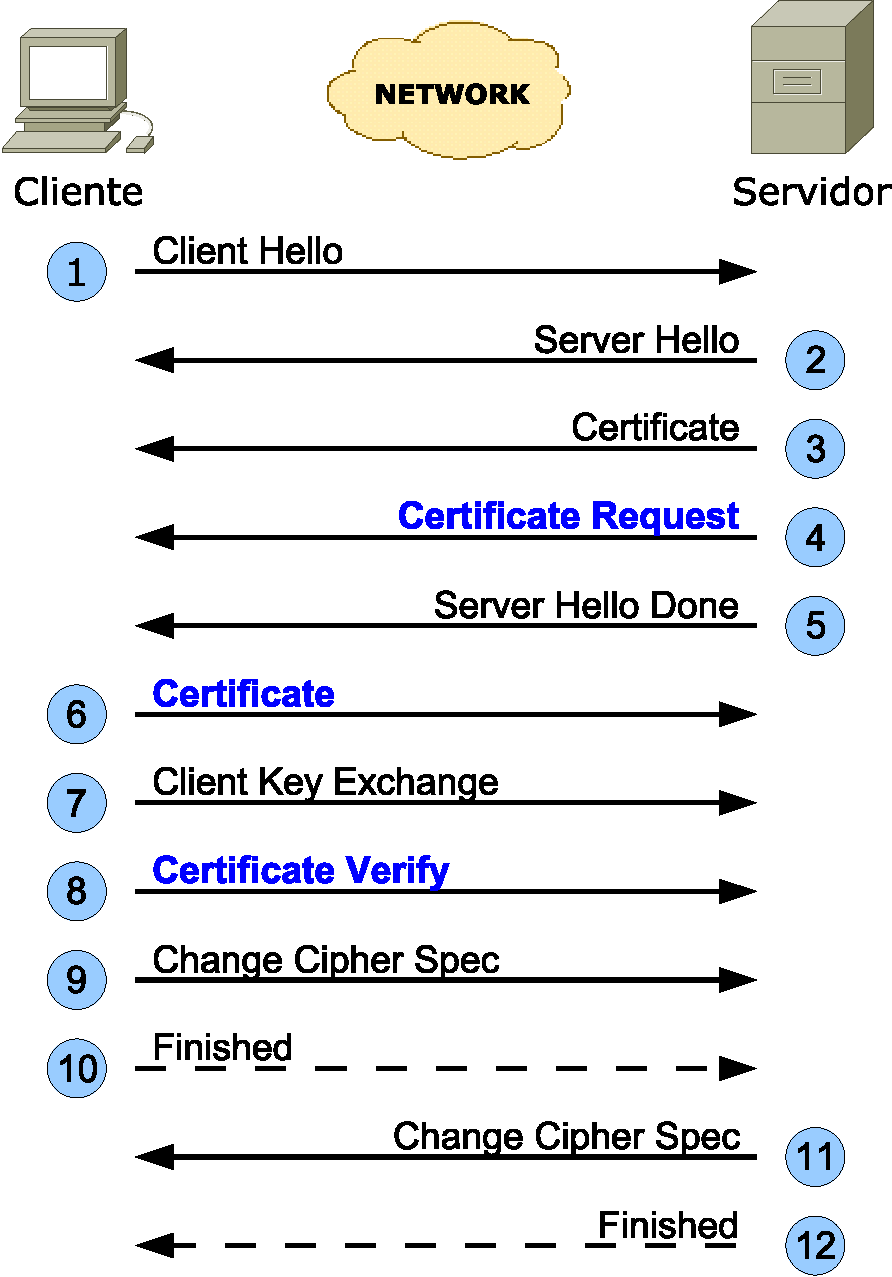
\includegraphics[scale=0.5]{fig/hs_mutual_auth}
    \caption{\emph{Handshake} completo com autenticação mútua}
    \label{fig:hs_mutual_auth}
\end{figure}

A Tabela~\vref{tab:hs_mutual_auth} resume as mensagens adicionais destacadas em negrito na
Figura~\vref{fig:hs_mutual_auth}.

\begin{table}[htp]
    \begin{center}
    \caption{\emph{Handshake} completo com autenticação mútua}
    \label{tab:hs_mutual_auth}
    \begin{tabular}{@{}cp{15cm}@{}} \toprule
    \tm{\#} & \tm{Descrição} \\ \midrule
4 &
O servidor solicita ao cliente que envie o seu certificado X.509. A mensagem
\tlsHsCr inclui uma lista das \acsp{CA} aceitáveis pelo servidor. \\
\addlinespace
6 &
O cliente envia o seu certificado e todos os eventuais certificados
intermediários (não raiz). \\
\addlinespace
8 &
Adicionalmente o cliente precisa enviar uma prova de autenticidade,
comprovando que possui a chave privada correspondente à chave pública
incluída no seu certificado. \\ \bottomrule
    \end{tabular}
    \end{center}
\end{table}

\subsubsection{\emph{Handshake} abreviado}

Esse mecanismo, denominado pela especificação de \emph{Session Resumption},
permite a restauração de uma sessão TLS negociada anteriormente, reduzindo todo
o \emph{handshake} a apenas 6 breves mensagens e dispensando todo esforço
computacional necessário para estabelecer uma nova conexão TLS. A
Tabela~\vref{tab:hs_resumed} descreve as principais mensagens que determinam a
restauração de uma sessão, cujo processo completo encontra-se ilustrado na
Figura~\vref{fig:hs_resumed}.

\begin{figure}[htb]
    \centering
        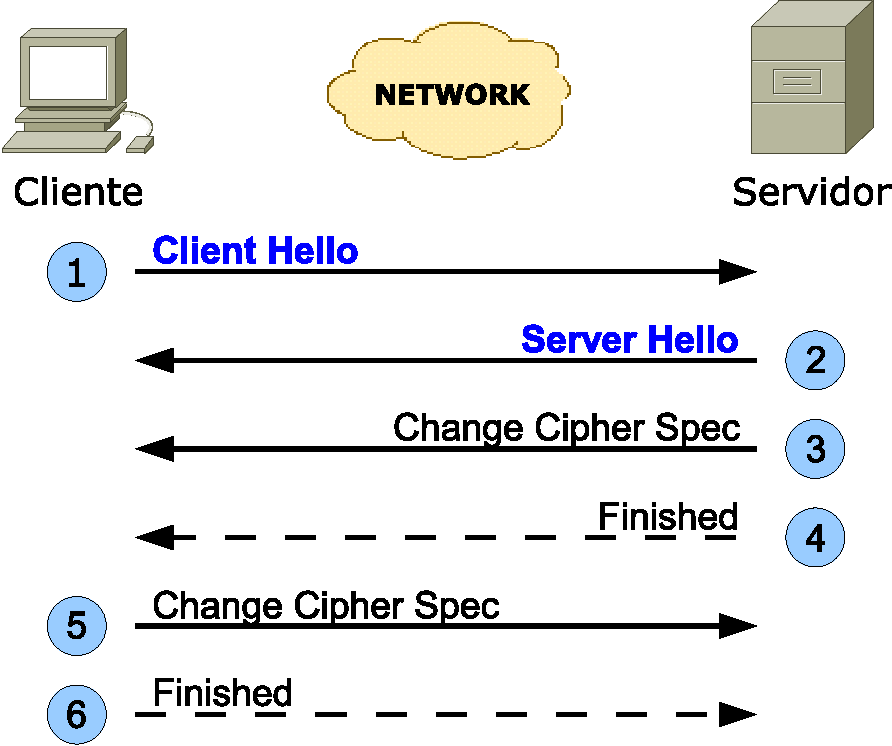
\includegraphics[scale=0.50]{fig/hs_resumed}
    \caption{\emph{Handshake} abreviado}
    \label{fig:hs_resumed}
\end{figure}

\begin{table}[htp]
    \centering
    \caption{\emph{Handshake} abreviado}
    \label{tab:hs_resumed}
    \begin{tabular}{@{}lp{15cm}@{}} \toprule
        \tm{\#} & \tm{Descrição} \\ \midrule
1 &
O cliente envia a mensagem \tlsHsCh contendo todos os parâmetros necessários para o
estabelecimento de uma nova sessão, mas inclui o identificador de sessão (\emph{``Session ID''}) extraído
da \tlsHsSh enviada por este servidor em uma sessão anterior. \\
\addlinespace
2 &
Servidor responde com \tlsHsSh contendo o mesmo identificador presente na \tlsHsCh, sinalizando
que a sessão será restaurada. \\ \bottomrule
    \end{tabular}
\end{table}
